\documentclass[11pt,a4paper]{article}

\usepackage{amsmath,amssymb,amsfonts}
\usepackage[margin=2.5cm]{geometry}
\usepackage{bm}
\usepackage{hyperref}
\usepackage{booktabs}
\usepackage{tikz}
\usetikzlibrary{arrows.meta,positioning,shapes.geometric}

\newcommand{\hlm}{h_{\ell m}}
\newcommand{\hcp}{h^{\mathrm{cp}}_{\ell m}}
\newcommand{\Alm}{A_{\ell m}}
\newcommand{\philm}{\phi_{\ell m}}
\newcommand{\Ylm}{{}^{-2}Y_{\ell m}}
\newcommand{\Dlm}{D^\ell_{mm'}}
\newcommand{\veclambda}{\bm{\lambda}}
\newcommand{\vecchi}{\vec{\chi}}

\title{General Waveform Decomposition for Neural Network Emulation}
\author{Jim Emulators Project}
\date{December 2025}

\begin{document}
\maketitle

\begin{abstract}
We present a general framework for neural network emulation of gravitational waveforms that can accommodate arbitrary physical complexity: precession, higher modes, and eccentricity. We clarify which aspects of the standard decomposition are coordinate choices versus restrictive physical assumptions, and propose a neural network architecture that learns the optimal frame decomposition end-to-end without requiring external Euler angle extraction.
\end{abstract}

\tableofcontents
\newpage

%%%%%%%%%%%%%%%%%%%%%%%%%%%%%%%%%%%%%%%%%%%%%%%%%%%%%%%%%%%%%%%%%%%%%%%%%%%%%%%
\section{Introduction}
%%%%%%%%%%%%%%%%%%%%%%%%%%%%%%%%%%%%%%%%%%%%%%%%%%%%%%%%%%%%%%%%%%%%%%%%%%%%%%%

Existing neural network emulators for gravitational waveforms make simplifying assumptions that limit their generality:
\begin{itemize}
    \item \textbf{mlgw\_NN} \cite{mlgw_nn}: Assumes aligned spins (non-precessing) and circular orbits
    \item \textbf{SEOBNN} \cite{seobnn}: Assumes single-spin systems ($\vecchi_2 = 0$), conjugate mode symmetry in the coprecessing frame, and circular orbits
    \item \textbf{SEOBNRE\_AI} \cite{seobnre_ai}: Includes eccentricity but only models the dominant $(2,2)$ mode with aligned spins
\end{itemize}

This document presents a framework that can accommodate any level of complexity, and addresses practical concerns about deploying such a framework on arbitrary waveform models.

%%%%%%%%%%%%%%%%%%%%%%%%%%%%%%%%%%%%%%%%%%%%%%%%%%%%%%%%%%%%%%%%%%%%%%%%%%%%%%%
\section{General Decomposition}
%%%%%%%%%%%%%%%%%%%%%%%%%%%%%%%%%%%%%%%%%%%%%%%%%%%%%%%%%%%%%%%%%%%%%%%%%%%%%%%

\subsection{Spherical Harmonic Expansion}

The gravitational wave strain observed at angles $(\iota, \varphi_0)$ from the source is expanded in spin-weighted spherical harmonics:
\begin{equation}
    \boxed{
    h(t; \veclambda; \iota, \varphi_0) = \sum_{\ell=2}^{\ell_{\max}} \sum_{m=-\ell}^{+\ell} \hlm(t; \veclambda) \, \Ylm(\iota, \varphi_0)
    }
    \label{eq:spherical_harmonic}
\end{equation}
where $\Ylm$ are the spin $-2$ weighted spherical harmonics, and $\veclambda$ denotes the \emph{intrinsic} parameter space.

\subsection{Intrinsic vs Extrinsic Parameters}
\label{sec:intrinsic_extrinsic}

A crucial feature of the decomposition \eqref{eq:spherical_harmonic} is that it separates parameters into two classes:

\paragraph{Intrinsic parameters $\veclambda$:} Properties of the source that affect the mode functions $\hlm(t)$:
\begin{equation}
    \veclambda = \{q, \, \chi_{1x}, \chi_{1y}, \chi_{1z}, \, \chi_{2x}, \chi_{2y}, \chi_{2z}, \, e_0, \, \ldots\}
    \label{eq:intrinsic_params}
\end{equation}
where $q = m_1/m_2$ is the mass ratio, $\vecchi_1, \vecchi_2$ are the dimensionless spin vectors, and $e_0$ is the orbital eccentricity.

\paragraph{Extrinsic parameters:} Properties that affect only how the modes combine or scale:
\begin{itemize}
    \item \textbf{Inclination $\iota$}: Enters only through $\Ylm(\iota, \varphi_0)$
    \item \textbf{Reference phase $\varphi_0$}: Enters only through $\Ylm(\iota, \varphi_0)$
    \item \textbf{Luminosity distance $d_L$}: Scales amplitude as $h \propto 1/d_L$
    \item \textbf{Polarisation angle $\psi$}: Rotates $h_+, h_\times$ at the detector
\end{itemize}

\paragraph{Implication for emulation:} The neural network only needs to learn the intrinsic modes $\hlm(t; \veclambda)$. Extrinsic parameters are handled analytically at inference time via the known spherical harmonic functions. One trained model works for all viewing angles.

\subsection{Coprecessing Frame Decomposition}

For precessing systems, we decompose each inertial-frame mode into coprecessing-frame modes via a time-dependent rotation:
\begin{equation}
    \boxed{
    \hlm(t; \veclambda) = \sum_{m'=-\ell}^{+\ell} \Dlm\bigl(\alpha(t), \beta(t), \gamma(t); \veclambda\bigr) \, h^{\mathrm{cp}}_{\ell m'}(t; \veclambda)
    }
    \label{eq:coprecessing}
\end{equation}
where $\Dlm$ are the Wigner D-matrices parameterised by Euler angles $\{\alpha(t), \beta(t), \gamma(t)\}$ that track the evolution of the orbital angular momentum $\hat{L}(t)$.

\subsection{Amplitude--Phase Decomposition}

Each coprecessing mode is decomposed into amplitude and phase:
\begin{equation}
    \boxed{
    \hcp(t; \veclambda) = \Alm(t; \veclambda) \, e^{i\philm(t; \veclambda)}
    }
    \label{eq:amp_phase}
\end{equation}

This decomposition is advantageous because $\Alm(t)$ and $\philm(t)$ are smooth functions that are easier for neural networks to learn than the oscillatory complex waveform.

%%%%%%%%%%%%%%%%%%%%%%%%%%%%%%%%%%%%%%%%%%%%%%%%%%%%%%%%%%%%%%%%%%%%%%%%%%%%%%%
\section{What is a Coordinate Choice vs a Restrictive Assumption}
%%%%%%%%%%%%%%%%%%%%%%%%%%%%%%%%%%%%%%%%%%%%%%%%%%%%%%%%%%%%%%%%%%%%%%%%%%%%%%%

\subsection{Coordinate Choices (Not Restrictive)}

The following are \emph{coordinate transformations} that can be applied to any waveform without loss of generality:

\begin{enumerate}
    \item \textbf{Spherical harmonic expansion} \eqref{eq:spherical_harmonic}: Always valid for any radiation field.

    \item \textbf{Coprecessing frame rotation} \eqref{eq:coprecessing}: This is just a time-dependent rotation of coordinates. The coprecessing frame is defined by tracking $\hat{L}(t)$, which exists for any binary orbit. The transformation is invertible and lossless.

    \item \textbf{Amplitude--phase decomposition} \eqref{eq:amp_phase}: Any complex function can be written in polar form.
\end{enumerate}

\subsection{Restrictive Assumptions}

The following are \emph{physical approximations} that limit the class of waveforms that can be accurately represented:

\begin{enumerate}
    \item \textbf{Conjugate symmetry in the inertial frame} (aligned-spin assumption):
    \begin{equation}
        h_{\ell,-m}(t; \veclambda) = (-1)^\ell h^*_{\ell m}(t; \veclambda)
        \label{eq:conjugate_inertial}
    \end{equation}
    This holds only for non-precessing systems with aligned spins.

    \item \textbf{Conjugate symmetry in the coprecessing frame}:
    \begin{equation}
        h^{\mathrm{cp}}_{\ell,-m}(t; \veclambda) = (-1)^\ell \bigl(h^{\mathrm{cp}}_{\ell m}(t; \veclambda)\bigr)^*
        \label{eq:conjugate_coprec}
    \end{equation}
    This approximation assumes the coprecessing-frame waveform looks like an aligned-spin waveform. It works well for mild precession but breaks down for strongly precessing systems.

    \item \textbf{Single-spin assumption} ($\vecchi_2 = 0$): Reduces the parameter space but excludes double-spin systems.

    \item \textbf{Circular orbit assumption} ($e_0 = 0$): Excludes eccentric binaries.
\end{enumerate}

\subsection{Summary Table}

\begin{table}[h]
\centering
\begin{tabular}{lcc}
\toprule
\textbf{Component} & \textbf{Type} & \textbf{Always Valid?} \\
\midrule
Spherical harmonic expansion & Coordinate choice & Yes \\
Coprecessing frame rotation & Coordinate choice & Yes \\
Amplitude/phase split & Coordinate choice & Yes \\
\midrule
Conjugate symmetry (inertial) & Approximation & No (aligned spin only) \\
Conjugate symmetry (coprecessing) & Approximation & No (mild precession only) \\
Single spin & Approximation & No \\
Circular orbits & Approximation & No \\
\bottomrule
\end{tabular}
\caption{Classification of decomposition components.}
\label{tab:assumptions}
\end{table}

%%%%%%%%%%%%%%%%%%%%%%%%%%%%%%%%%%%%%%%%%%%%%%%%%%%%%%%%%%%%%%%%%%%%%%%%%%%%%%%
\section{Where Different Physics Enters}
%%%%%%%%%%%%%%%%%%%%%%%%%%%%%%%%%%%%%%%%%%%%%%%%%%%%%%%%%%%%%%%%%%%%%%%%%%%%%%%

\subsection{Precession}

Precession is handled by the coprecessing frame transformation. The Euler angles $\alpha(t), \beta(t), \gamma(t)$ encode the precession dynamics---the time-dependent orientation of the orbital plane.

\textbf{Key point}: The coprecessing frame transformation \emph{handles} precession but doesn't \emph{add} it. If the underlying modes don't contain precession physics, the transformation is trivial ($\Dlm \to \delta_{mm'}$).

\subsection{Eccentricity}

Eccentricity affects the \emph{intrinsic} time evolution of the modes. It enters through:
\begin{enumerate}
    \item Mode amplitudes $\Alm(t)$: Eccentric orbits produce amplitude modulations at the orbital frequency
    \item Mode phases $\philm(t)$: More complex orbital phase evolution with periastron advance
    \item Euler angles $\alpha(t), \beta(t), \gamma(t)$: Precession dynamics couple to eccentricity
    \item The coprecessing frame definition: $\hat{L}(t)$ has more complex trajectory
\end{enumerate}

\textbf{Key point}: Eccentricity cannot be added by coordinate transformations. It must be present in the underlying waveform model being emulated.

\subsection{Implications for IMRPhenomX Family}

\begin{itemize}
    \item \textbf{IMRPhenomXHM}: Non-precessing, higher modes, circular. Can serve as coprecessing modes.
    \item \textbf{IMRPhenomXPHM}: Uses XHM as coprecessing modes + Euler angle rotation. Precessing, higher modes, circular.
    \item \textbf{Neither has eccentricity}: To emulate eccentric waveforms, one must start from an eccentric model (e.g., SEOBNRE, TEOBResumS-GIOTTO).
\end{itemize}

%%%%%%%%%%%%%%%%%%%%%%%%%%%%%%%%%%%%%%%%%%%%%%%%%%%%%%%%%%%%%%%%%%%%%%%%%%%%%%%
\section{The Euler Angle Extraction Problem}
%%%%%%%%%%%%%%%%%%%%%%%%%%%%%%%%%%%%%%%%%%%%%%%%%%%%%%%%%%%%%%%%%%%%%%%%%%%%%%%

\subsection{The Practical Challenge}

For emulation, we assume the input is a ``black box'' waveform code that outputs only inertial-frame quantities:
\begin{equation}
    \text{Code}: \quad \veclambda \mapsto \{h_+(t), h_\times(t)\} \quad \text{or} \quad \veclambda \mapsto \{\hlm(t)\}
\end{equation}

The coprecessing modes and Euler angles are \emph{not} provided. Some codes (e.g., SEOBNRv4PHM in LALSuite) do expose these internally, but this cannot be assumed in general.

\subsection{Non-Uniqueness of the Coprecessing Frame}

There is no single ``correct'' definition of the coprecessing frame. Valid choices include:
\begin{itemize}
    \item \textbf{$L$-frame}: Track instantaneous orbital angular momentum $\hat{L}(t)$
    \item \textbf{$J$-frame}: Align with total angular momentum $\hat{J}$ at reference time
    \item \textbf{Quadrupole-preferred frame}: Minimise power in non-$(2,\pm2)$ modes
    \item \textbf{Minimal rotation frame}: Impose $\dot{\gamma} = -\dot{\alpha}\cos\beta$
\end{itemize}

Different conventions give different Euler angles and coprecessing modes, though all are valid coordinate choices.

\subsection{Classical Extraction Methods}

If one chooses to extract Euler angles from inertial-frame waveforms, established methods exist:
\begin{enumerate}
    \item \textbf{Dominant eigenvector method}: Find the frame maximising power in $(2,\pm2)$
    \item \textbf{Phase gradient method}: Extract from the $(2,2)$ mode phase evolution
    \item \textbf{Optimisation}: Minimise some cost function over rotation parameters
\end{enumerate}

These methods work but introduce preprocessing complexity and convention dependence.

%%%%%%%%%%%%%%%%%%%%%%%%%%%%%%%%%%%%%%%%%%%%%%%%%%%%%%%%%%%%%%%%%%%%%%%%%%%%%%%
\section{Neural Network Architecture Options}
%%%%%%%%%%%%%%%%%%%%%%%%%%%%%%%%%%%%%%%%%%%%%%%%%%%%%%%%%%%%%%%%%%%%%%%%%%%%%%%

We consider three architectural approaches for learning precessing waveforms.

\subsection{Option 1: Extract Then Learn}

\begin{enumerate}
    \item Use classical algorithms to extract Euler angles from training waveforms
    \item Train separate neural networks for coprecessing modes and Euler angles
    \item At inference, predict both and combine via Wigner rotation
\end{enumerate}

\textbf{Pros}: Physics-informed, interpretable, follows literature \\
\textbf{Cons}: Extraction is non-unique, adds preprocessing step, convention-dependent

\subsection{Option 2: Learn Inertial Modes Directly}

\begin{enumerate}
    \item Skip decomposition entirely
    \item Train neural network: $\veclambda \mapsto \hlm(t)$ in inertial frame
\end{enumerate}

\textbf{Pros}: Simple pipeline, no extraction needed \\
\textbf{Cons}: Inertial modes have fast precession oscillations, much harder to learn, requires larger networks

\subsection{Option 3: Learn Frame Decomposition End-to-End (Recommended)}

Build the Wigner rotation into the network architecture:

\begin{center}
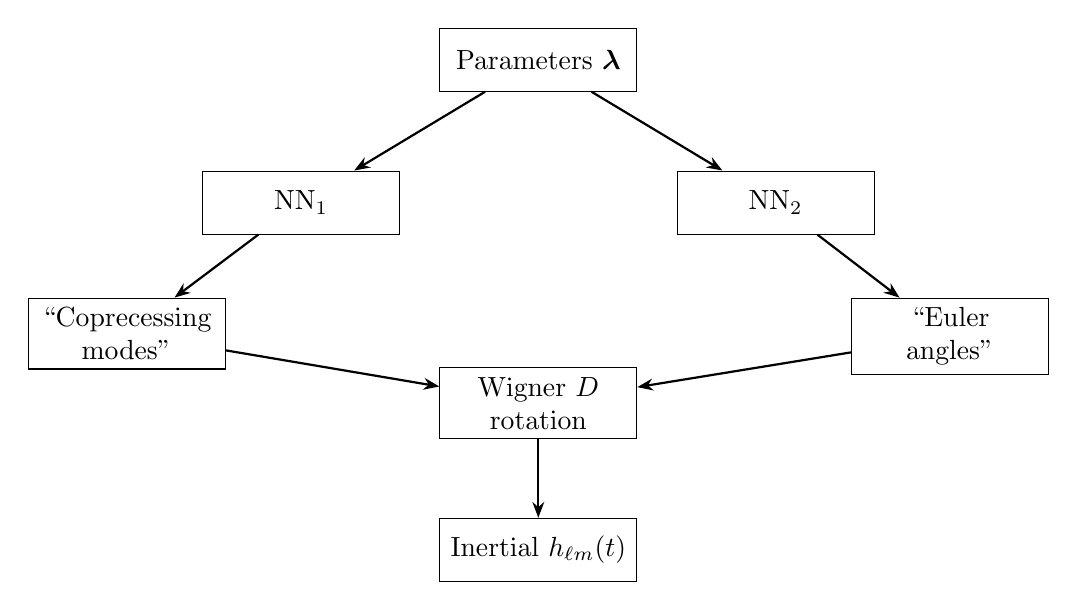
\begin{tikzpicture}[
    node distance=1.5cm,
    box/.style={rectangle, draw, minimum width=2.5cm, minimum height=0.8cm, align=center},
    arrow/.style={-{Stealth[length=2mm]}, thick}
]
    \node[box] (params) {Parameters $\veclambda$};
    \node[box, below left=1cm and 0.5cm of params] (nn1) {NN$_1$};
    \node[box, below right=1cm and 0.5cm of params] (nn2) {NN$_2$};
    \node[box, below left=0.8cm and -0.3cm of nn1] (modes) {``Coprecessing\\modes''};
    \node[box, below right=0.8cm and -0.3cm of nn2] (euler) {``Euler\\angles''};
    \node[box, below=3.5cm of params] (wigner) {Wigner $D$\\rotation};
    \node[box, below=1cm of wigner] (output) {Inertial $\hlm(t)$};

    \draw[arrow] (params) -- (nn1);
    \draw[arrow] (params) -- (nn2);
    \draw[arrow] (nn1) -- (modes);
    \draw[arrow] (nn2) -- (euler);
    \draw[arrow] (modes) -- (wigner);
    \draw[arrow] (euler) -- (wigner);
    \draw[arrow] (wigner) -- (output);
\end{tikzpicture}
\end{center}

The loss function is computed on the inertial-frame output:
\begin{equation}
    \mathcal{L} = \sum_{\ell m} \left\| \hlm^{\text{pred}}(t) - \hlm^{\text{true}}(t) \right\|^2
\end{equation}

\textbf{Key features}:
\begin{itemize}
    \item No external Euler angle extraction needed
    \item Physics structure (rotation equivariance) is built into architecture
    \item Network learns whatever internal decomposition works best
    \item The learned ``Euler angles'' are latent variables---they need not match any standard convention
    \item Works with any code that outputs $\hlm(t)$ in the inertial frame
\end{itemize}

\textbf{Pros}: General, no preprocessing, physics-informed architecture \\
\textbf{Cons}: More complex architecture, learned angles may not be interpretable

\subsection{Comparison}

\begin{table}[h]
\centering
\begin{tabular}{lccc}
\toprule
\textbf{Criterion} & \textbf{Option 1} & \textbf{Option 2} & \textbf{Option 3} \\
\midrule
External extraction needed & Yes & No & No \\
Convention dependence & Yes & No & No \\
Physics structure exploited & Yes & No & Yes \\
Interpretable intermediates & Yes & N/A & No \\
Network complexity & Medium & High & Medium \\
Training difficulty & Medium & Hard & Medium \\
\bottomrule
\end{tabular}
\caption{Comparison of architectural options.}
\label{tab:options}
\end{table}

%%%%%%%%%%%%%%%%%%%%%%%%%%%%%%%%%%%%%%%%%%%%%%%%%%%%%%%%%%%%%%%%%%%%%%%%%%%%%%%
\section{Architecture Requirements}
%%%%%%%%%%%%%%%%%%%%%%%%%%%%%%%%%%%%%%%%%%%%%%%%%%%%%%%%%%%%%%%%%%%%%%%%%%%%%%%

\subsection{Without Conjugate Symmetry}

For a fully general emulator covering $\ell \leq \ell_{\max}$ without assuming conjugate symmetry:

\begin{table}[h]
\centering
\begin{tabular}{lcc}
\toprule
\textbf{Component} & \textbf{Count} & \textbf{Notes} \\
\midrule
Coprecessing amplitudes $\Alm(t)$ & $\sum_{\ell=2}^{\ell_{\max}} (2\ell + 1)$ & All $m \in [-\ell, +\ell]$ \\
Coprecessing phases $\philm(t)$ & $\sum_{\ell=2}^{\ell_{\max}} (2\ell + 1)$ & All $m \in [-\ell, +\ell]$ \\
Euler angles & 3 & $\alpha(t), \beta(t), \gamma(t)$ \\
\bottomrule
\end{tabular}
\caption{Neural network outputs required for general emulation.}
\label{tab:surrogates}
\end{table}

For $\ell_{\max} = 4$ (modes up to $(4,\pm4)$): $5 + 7 + 9 = 21$ complex modes $\times 2$ (amp/phase) $+ 3$ Euler angles $= 45$ output functions.

\subsection{With Conjugate Symmetry (if applicable)}

If conjugate symmetry can be assumed (aligned spins or mild precession), only $m \geq 0$ modes need to be modelled, roughly halving the outputs.

%%%%%%%%%%%%%%%%%%%%%%%%%%%%%%%%%%%%%%%%%%%%%%%%%%%%%%%%%%%%%%%%%%%%%%%%%%%%%%%
\section{Summary}
%%%%%%%%%%%%%%%%%%%%%%%%%%%%%%%%%%%%%%%%%%%%%%%%%%%%%%%%%%%%%%%%%%%%%%%%%%%%%%%

The complete general decomposition is:
\begin{align}
    h(t; \veclambda; \iota, \varphi_0) &= \sum_{\ell, m} \hlm(t; \veclambda) \, \Ylm(\iota, \varphi_0) \label{eq:summary1} \\[0.5em]
    \hlm(t; \veclambda) &= \sum_{m'} \Dlm\bigl(\alpha, \beta, \gamma; t, \veclambda\bigr) \, h^{\mathrm{cp}}_{\ell m'}(t; \veclambda) \label{eq:summary2} \\[0.5em]
    \hcp(t; \veclambda) &= \Alm(t; \veclambda) \, e^{i\philm(t; \veclambda)} \label{eq:summary3}
\end{align}

\textbf{Key points}:
\begin{enumerate}
    \item Inclination and reference phase are extrinsic---handled analytically via spherical harmonics.
    \item The coprecessing frame decomposition is a coordinate choice, not a restrictive assumption.
    \item Conjugate symmetry (in either frame) IS a restrictive assumption.
    \item Eccentricity must be in the underlying model---it cannot be added by coordinate transformations.
    \item For practical emulation, we recommend learning the frame decomposition end-to-end (Option 3), avoiding the need for external Euler angle extraction.
\end{enumerate}

%%%%%%%%%%%%%%%%%%%%%%%%%%%%%%%%%%%%%%%%%%%%%%%%%%%%%%%%%%%%%%%%%%%%%%%%%%%%%%%
\begin{thebibliography}{9}

\bibitem{mlgw_nn}
T.~Grimbergen, S.~Schmidt, C.~Kalaghatgi, C.~Van Den Broeck,
``Generating Higher Order Modes from Binary Black Hole mergers with Machine Learning,''
arXiv:2402.06587 (2024).

\bibitem{seobnn}
L.~M.~Thomas, G.~Pratten, P.~Schmidt,
``Accelerating multimodal gravitational waveforms from precessing compact binaries with artificial neural networks,''
arXiv:2205.14066 (2022).

\bibitem{seobnre_ai}
R.~Shi et al.,
``Rapid eccentric spin-aligned binary black hole waveform generation based on deep learning,''
arXiv:2411.14893 (2024).

\end{thebibliography}

\end{document}
